\chapter{Implementation}
\label{chapter:implementation}

%\section{Implementation Options}
%Neste secção devem apresentar as opções de implementação que tinham ao vosso
%dispor, avaliá-las e justificar a escolha que realizaram. Isto pode englobar:
%\begin{itemize}
%    \item Simuladores
%    \item Linguagens e ambientes de programação
%    \item Sistemas operativos
%    \item Hardware
%\end{itemize}
%Fica sempre bem na avaliação colocar uma tabela com as características
%pretendidas e as que são satisfeitas pelas várias opções (tipo catálogo com as
%características dos automóveis). A escolha deve surgir naturalmente, com base na
%opção que tem mais cruzes\ldots

%\section{Architecture}
%Nesta secção devem explicar como implementaram a vossa solução, apresentando
%as simplificações que efectuaram, face ao modelo inicialmente previsto. As
%simplificações devem ser devidamente justificadas. Se for possível, devem indicar
%que estas não põem em causa as contribuições da tese.
%Podem ainda descrever os principais problemas que tiveram e a forma como os
%abordaram e resolveram.

%Se estiverem a usar um simulador devem:

%\begin{itemize}
%    \item explicar o funcionamento do simulador
%    \item explicar as alterações e modelos que desenvolveram no simulador e que permitem validar a vossa ideia
%\end{itemize}

%Se estiveram a desenvolver SW, sem simulador devem:
%\begin{itemize}
%    \item explicar os módulos, interfaces, estruturas de dados, etc\ldots
%\end{itemize}

%Sempre que possível, ilustrem a arquitectura com figuras que demonstrem a
%evolução face à arquitectura da secção anterior. Isto é, usem as figuras anteriores
%e façam as modificações necessárias à obtenção da arquitectura do protótipo.
%\ldots

In this chapter we are going to present our implementation choices, the difficulties that we have faced and the strategies available to overcome them.

To this end, we are going to present and explain our database model, how we have improved it and how this model can help us reach our goals. 

Subsequently, we are going to describe our signaling protocol which will make it possible to use the \ac{WebRTC}'s functionalities in order to implement our system's streaming features.

With the model and signaling protocol defined we are prepared to show the multiple approaches we have followed in order to implement stream recording, their drawbacks and our choices.

Then are going to describe how we show hyper-content to users, namely the multiple ways to create hyper-content and the algorithm behind the user interface synchronization, the security flaws of our content displaying mechanism and a possible solution to overcome vulnerabilities. 

Not less important we also are going to describe how we have implemented our application time-line and the functionalities above it such as time manipulation and annotations management. Among other different functionalities we also are going to describe how we perform stream composition, synchronization of our collaborative text editor and implementation of our instant messenger.

Lastly, we are going to describe the deployment of our solution in respect to the hardware that we have used and the software installed onto it.


%RP antes desta secção fala um introdução ao capítulo a explicar o que vai ser apresentado.
%HR done

\section{Data Model}
The data model is a critical component of our solution, as a badly designed model can imply serious difficulties when implementing new features that are not part of the plans. During the course of this project, we had to redesign the model more than once in order to support new features.

%RP devias começar com um overview dos dados que é necessário guardar para a aplicação
%RP ao apresentar o modelo falas de coisas como mensagens para grupos, mas ainda não sabemos nada disso. Na arquitectura, devias falar da concepção, do modelo de comunicação. Que tens utilizadores, grupos, mensagens, chats, convites, etc...
%HR não meti na arquitectura mas adicionei a linha seguinte

In order to offer all the functionalities that we promise, some information about objects must be persistent such as users, groups,relations among users, group memberships, messages, hyper-content, recordings and collaborative editor state.

\subsection {Schema representation}
    \emph{MongoDB} has a slightly different terminology from relational databases. The first big difference is instead of having tables \emph{MongoDB} stores its objects on collections. The analogous data structure to the table row is a document.

    Each \emph{MongoDB} document is represented by a \emph{JSON} object and, as a result, each document may have different attributes within a collection. Needless to say that, by following this approach we do not need to create the collections with a well predefined schema. In fact, we do not need to define it at all but, for reasons of coherence and organization, we represent our database collections as they would have a predefined schema by following the same document structure as we will present in this section.
    %RP a última frase é confusa. O que queres dizer? Reescreve
    %HR está melhor?

    Similarly to relational databases, \emph{MongoDB} requires a primary key (typically of type \emph{ObjectId} and named \emph{"\_id"}) for each document, which is automatically assigned if not specified. 

    In order to define \emph{foreign keys}, we just store them as \emph{ObjectId}s if and only if the foreign keys point to documents within a unique collection, otherwise we need an additional attribute to specify which collection is the \emph{foreign key} pointing at.

    In respect to attributes nullability, \emph{MongoDB} does not enforce a document's attribute to have a not null value, although, for sake of good functionality, we perform those constraints validation programmatically and as such we also represent them in our schema.
    
    An example of schema representation can be seen on Table \ref{table:schema}.

\begin{table}
\centering
\caption{Schema representation}
\label{table:schema}
    \begin{tabular}{|ll|}
        \hline
        \multicolumn{2}{|c|}{\textbf{Collection name}}            \\ \hline
        $\Diamondblack$ \underline{\_id (primary key)} & ObjectId \\ 
        $\medbullet$ Not nullable property name & Property type   \\ 
        $\medcirc$ Nullable property name       & Property type   \\
        $\medcirc$ Reference to document        & ObjectId        \\
        $\medbullet$ Embedded document          & Document        \\ 
        $\medbullet$ Embedded list              & List[Type]      \\ \hline
    \end{tabular}
\end{table}

\subsection {Generic model}

For designing our model we have taken into account generic programming techniques. We observed that operations like searching for an object were quite repeated across different types of objects. 

Our first decision for our model, in order to avoid repeated code, was the isolation of the object's attributes from themselves, so we could apply the search operation to a set of attributes independently of the object type. To this generic set of properties we call data (Table \ref{table:generic}) and each object of this type has a reference to the owner, which is a unique identification number.

\begin{table}
\centering
\caption{Generic data model}
\label{table:generic}
    \begin{tabular}{cc}
        \begin{tabular}{|ll|}
            \hline
            \multicolumn{2}{|c|}{\textbf{Data}}          \\ \hline
            $\Diamondblack$ \underline{\_id} & ObjectId  \\ 
            $\medbullet$ owner          & ObjectId       \\ 
            $\medbullet$ properties    & List[Attribute] \\ 
            $\medcirc$ searchableValues & List[Text]     \\ \hline
        \end{tabular}
        \begin{tabular}{|ll|}
            \hline
            \multicolumn{2}{|c|}{\textbf{Attribute}}     \\ \hline
            $\medbullet$ key            & Text           \\ 
            $\medcirc$ value            & Object         \\ 
            $\medbullet$ identifiable   & Boolean        \\ 
            $\medcirc$ readPermissions  & List[ObjectId] \\ 
            $\medcirc$ writePermissions & List[ObjectId] \\ \hline
        \end{tabular}    
    \end{tabular}
\end{table}

The owner's identification number by itself is not sufficient to identify an object, as objects from different types can have the same identification number. In order to solve this problem, when an object is created, its correspondent data must contain the owner's object type. 
%RP mas o _id é apresentado com sendo uma chave primária na figura 4.2, logo única!
%HR "The owner's identification number" corriji, não me referia ao "_id"

Whenever an attribute is created, its name, value and indentifiability must be specified. The set of objects that can read and write that attribute must also be defined. 
In regard to our permission mechanism, if the read or write sets are not specified we assume the attribute is readable and writable by everyone. Conversely if the read and write sets are empty, nobody is allowed to read or write the attribute. Implicitly, if an entity can write an attribute, it can also read it.

In particular, if all attributes were searchable, it could be simple to search for attributes that could reveal sensible information about an object. For example if we consider that a user could have a health related attribute, searching by a disease would reveal which users could suffer from a certain disease. The leak of that kind of information could, for instance, change the agreement between users and health insurance companies. For this reason only the specified attributes as searchable will be taken into account when performing keyword searches.
%RP era melhor que o exemplo fosse relativo à tua aplicação e não algo abstracto como saúde.
%RP Dás permissões de leitura e escrita a objectos. Normalmente é a utilizadores. Explicar relação. Assumo que sejam aqui referenciados apenas objectos que representam utilizadores

Another important attribute specification is the owner identifiability, which tells us if the attribute identifies the object. This specification lets us create abstract authentication services. For example a user can login into our system by providing any attribute that identifies himself, \emph{e.g.} the e-mail, but others are possible like the user name or cellphone number. 

Not less important, in order to get an object's properties efficiently, we have created an index over the \emph{owner} attribute. We have also created an index over the \emph{searchableValues} in order to improve the keyword search performance.

In summary, with this model we can perform search and identification of any kind of objects, as we will see on the following models. In particular, the \emph{user} and \emph{group} models are using this generic model for storing their attributes. 
% Not less important, attributes can specify aggregations of objects. For example, the user role is an aggregator property that within users it allows the identifaction of each one is administrator. This aggregation specification is independent from the object type, so it is possible to search for the administrative role and return users and groups of users that contains that property. <= [currently this operation is possible but it is not specified]


%RP antes de falares de cada modelo, que tal incluir uma figura com a relação entre os vários tipos de dados. Mesmo não sendo SQL, as relações existem conceptualmente e falas em chaves estrangeiras, pelo que tal figura faz sentido e ajuda a perceber.

\subsection{User model}

The user model is not tied to the user attributes (Table \ref{table:user}), the information maintained in this model is just used for authentication purposes. Passwords are not stored in plain text, instead we apply hashing and salting techniques \cite{password} in order to make it harder to decode the password by an attacker. Accordingly, we use \emph{SHA-1} and a random salt per user with 32 characters.
%RP Table x, Figure y, etc é sempre maiusculas.

\begin{table}
\centering
\caption{User model}
\label{table:user}
    \begin{tabular}{|ll|}
        \hline
        \multicolumn{2}{|c|}{\textbf{User}}         \\ \hline
        $\Diamondblack$ \underline{\_id}  & ObjectId  \\ 
        $\medbullet$ hash           & Text          \\ 
        $\medbullet$ salt      & Text               \\ \hline
    \end{tabular}
\end{table}

\subsection{Relation model}
% HR-FINAL - Sim isso, relações em geral, user-grupo, user-user, grupo-grupo, user-carro, user-escola... no fundo entidades, como está escrito

A relation between two entities $e_1$ and $e_2$ is represented by the pair $e_1\rightarrow e_2$ (Table \ref{table:relation}), where $e_1$ is the source and $e_2$ is the target. This relation is said to be bi-directional if and only if it also exists the relation $e_2\rightarrow e_1$.

\begin{table}
\centering
\caption{Relation model}
\label{table:relation}
    \begin{tabular}{|ll|}
        \hline
        \multicolumn{2}{|c|}{\textbf{Relation}}     \\ \hline
        $\Diamondblack$ \underline{\_id}  & ObjectId  \\ 
        $\medbullet$ source           & ObjectId    \\ 
        $\medbullet$ target      & ObjectId         \\ \hline
    \end{tabular}
\end{table}

A user can only interact with friends or with group members. In order to validate a friendship, both users must agree on that friendship, in other words it, there must exist a bi-directional relation between both users.

In order to improve the performance of queries over the \emph{Relation} collection we have created indexes on the \emph{source}, \emph{target} and also on the pair composed by both attributes.

\subsection{Group model}

A conference room, which is the environment where users communicate among themselves, is represented persistently by a group of participating entities (in general users but our system allow other types of entities). A conference room is composed by only online users and does not need to be stored on database.

A group is composed by an \emph{id}, \emph{inviteToken} and a \emph{visibility} as shown on Table \ref{table:group}.
Moreover, a group can be public or private. If the group is public, then it is visible to all users that maintain a friendship with a member of this group. If the group is private, then it is only visible to its members.


\begin{table}
\centering
\caption{Group model}
\label{table:group}
    \begin{tabular}{cc}
        \begin{tabular}{|ll|}
            \hline
            \multicolumn{2}{|c|}{\textbf{Group}}        \\ \hline
            $\Diamondblack$ \underline{\_id}  & ObjectId  \\ 
            $\medcirc$ inviteToken           & Text     \\ 
            $\medbullet$ visibility      & Text         \\ \hline
        \end{tabular}

        \begin{tabular}{|ll|}
            \hline
            \multicolumn{2}{|c|}{\textbf{GroupMembership}}  \\ \hline
            $\Diamondblack$ \underline{\_id}  & ObjectId      \\ 
            $\medbullet$ groupId            & ObjectId      \\ 
            $\medbullet$ userId & ObjectId                  \\ \hline
        \end{tabular}    
    \end{tabular}
\end{table}


The group membership is a special case of relation, where the target entity is always a group.
When a group is created, a group membership is automatically assigned to its creator.

Entities that have a membership with a group can create more memberships by sharing an invite token or by specifying new group members. This invite token is used to create an invite \ac{URL} that if shared with other users allow them to join the group. Invite tokens can be deleted or regenerated with a different value.
%RP isto quer dizer que quem tem o token se pode juntar ao grupo? Explicar. O que impede alguém de o partihar com outros?
%HR done

In order to improve performance of queries over \emph{GroupMembership} collection we have created indexes on the \emph{groupId}, \emph{userId} and also on the pair composed by both attributes.


\subsection{Message model}

A message is composed by its content, time of creation and source and target identification numbers (Table \ref{table:message}). The message's target could reference any object, but our application is only handling messages to groups.

\begin{table}
\centering
\caption{Message model}
\label{table:message}
    \begin{tabular}{|ll|}
        \hline
        \multicolumn{2}{|c|}{\textbf{Message}}      \\ \hline
        $\Diamondblack$ \underline{\_id}  & ObjectId  \\ 
        $\medbullet$ source           & ObjectId    \\ 
        $\medbullet$ target      & ObjectId         \\ 
        $\medbullet$ content      & Text            \\ \hline
    \end{tabular}
\end{table}

In order to query for recent messages for a given target, we use the oldest message's \emph{\_id}, which is sequential, in order to find messages with a newer \emph{\_id}.

In order to improve performance of queries over \emph{Relation} collection we have created indexes on the \emph{target} attribute and also on the pair composed by \emph{target} and \emph{\_id} attributes for finding and sorting the messages received by an entity more efficiently. 

%RP pela justificação não consigo perceber para que serve a chave no par target e _id
%HR in order to find recent messages (não tinha explicado)

\subsection{Hyper content model}

During a group conversation, it is possible to create time annotations for making it easy to access that time either for searching or sharing with other users.
A time annotation (Table \ref{table:hyper}) contains a title, the correspondent group identification number and the time itself.

The hyper content is used to synchronize content among users during a conversation. Table \ref{table:hyper} shows that every hyper content must have a start and ending time, the correspondent group identification number and the content itself, in the form of text. Beside those attributes, in order to perform queries over the \ac{HTML} contents with more precision, we have added an additional \emph{searchableContent} attribute. It contains just the searchable content extracted from the content, by excluding the \ac{HTML} tags and parameters using \emph{Jsoup}\footnote{\url{http://jsoup.org/} (Accessed April 11, 2016)}.

In the point o view of a user, a time annotation is just a simple way to associate a time stamp to a topic in order to make it easier to find. On the other hand, the hyper-content is more complete than time annotations, except they are not visible on the timeline. In addition to time annotations, hyper-contents have a duration and content that can be superimposed to video.

%RP explica melhor a diferença entre HyperContent e Time Annotation do ponto de vista do utilizador / funcionalidade proporcionada.
%HR done

\begin{table}
\centering
\caption{Hyper content model}
\label{table:hyper}
    \begin{tabular}{cc}
        \begin{tabular}{|ll|}
            \hline
            \multicolumn{2}{|c|}{\textbf{HyperContent}}  \\ \hline
            $\Diamondblack$ \underline{\_id}  & ObjectId \\ 
            $\medbullet$ groupId            & ObjectId   \\ 
            $\medbullet$ start              & Date       \\ 
            $\medbullet$ end                & Date       \\ 
            $\medbullet$ content            & Text       \\ 
            $\medbullet$ searchableContent  & Text       \\ \hline
        \end{tabular}

        \begin{tabular}{|ll|}
            \hline
            \multicolumn{2}{|c|}{\textbf{TimeAnnotation}}  \\ \hline
            $\Diamondblack$ \underline{\_id}  & ObjectId   \\ 
            $\medbullet$ groupId            & ObjectId     \\ 
            $\medbullet$ title & Text                      \\ 
            $\medbullet$ time & Date                       \\ \hline

        \end{tabular}    
    \end{tabular}
\end{table}

For example the content showed in Listing \ref{lst:jsoup} would produce the searchable content "Click here!".

\begin{minipage}{\linewidth}
\begin{lstlisting}[caption={Example of HTML content},label={lst:jsoup},language=JavaScript]
<div class="subtitle">
    <a href="/">Click here!</a>
</div>
\end{lstlisting}
\end{minipage}

In order to improve the performance of searching content and calculate interval intersections, we have created indexes over the following sequences of attributes: 

\begin{itemize}
\item{\emph{\{groupId,start,end\}} $\rightarrow$ for finding visible contents for a given time  within a group (intersections).}
\item{\emph{\{groupId,start\}} $\rightarrow$  for finding contents that starts after a given time within a group (for pre-loading).}
\item{\emph{\{groupId,searchableContent\}} $\rightarrow$ for searching contents by keywords within a group.}  
\end{itemize}

\subsection{Collaborative Content model}

Within a conversation, users can write documents collaboratively. As we can see in Table \ref{table:collaborative}, each document has a content and a reference to the correspondent group. 


\begin{table}
\centering
    \caption{Collaborative content model}
    \label{table:collaborative}
    \begin{tabular}{|ll|}
        \hline
        \multicolumn{2}{|c|}{\textbf{CollaborativeContent}} \\ \hline
        $\Diamondblack$ \underline{\_id}  & ObjectId        \\ 
        $\medbullet$ groupId            & ObjectId          \\ 
        $\medcirc$ content            & Text                \\ \hline
    \end{tabular}
\end{table}

In order to improve the performance of finding the group's content we have created and index over the \emph{groupId} attribute.

\subsection{Recording model}

During a conversation, users may allow sharing their web cameras. By doing so, their video is stored in recording chunks. Each chunk, described in Table \ref{table:recording}, represents an interval of time $T=\big[c^{start},c^{end}\big[$ of the video stream. It also contains the media's \ac{URL}, a reference to a group, an owner identification number and the correspondent \emph{WebSocket} session id.
    
    The media's \ac{URL} is the location where \emph{Kurento Repository} stores one chunk of video (including audio) which is used to playback on users demand.

    %RP ainda não tenho forma de perceber o que é o websocket session id. Nunca falaste de websockets antes, quanto mais disto! Nem do media URL, é gravado ou webrtc (dispositivo do utilizador)?
    
    In order to allow the same user to have different devices, storing just the \ac{URL} with an associated user id is not enough. In this case, one more parameter is needed to differentiate the different \emph{webSocket} sessions opened by the same user. For this reason we had to associate a random session identification number to each \emph{webSocket}.

\begin{table}
\centering
    \caption{Recording model}
    \label{table:recording}
    \begin{tabular}{cc}
        \begin{tabular}{|ll|}
            \hline
            \multicolumn{2}{|c|}{\textbf{RecordingInterval}}  \\ \hline
            $\Diamondblack$ \underline{\_id}  & ObjectId      \\ 
            $\medbullet$ groupId            & ObjectId        \\ 
             $\medbullet$ start             & Date            \\ 
            $\medbullet$ end                & Date            \\ \hline
        \end{tabular}   
        \begin{tabular}{|ll|}
            \hline
            \multicolumn{2}{|c|}{\textbf{RecordingChunk}}  \\ \hline
            $\Diamondblack$ \underline{\_id}  & ObjectId     \\ 
            $\medbullet$ groupId            & ObjectId     \\ 
            $\medbullet$ owner           & ObjectId        \\ 
            $\medbullet$ sessionId          & Text         \\
            $\medbullet$ start              & Date         \\ 
            $\medbullet$ end                & Date         \\ 
            $\medbullet$ url               & Text          \\ \hline
        \end{tabular}
    \end{tabular}
\end{table}



A set of chunks $S=[c_1,c_2,\ldots,c_n]$ is said continuous if $\forall c_i\in S, \exists c_j \in S$ where $j\neq i$ and $c_i^{start} = c_j^{end} \vee c_i^{end} = c_j^{start}$. 
A recording interval represents a continuous set of recording chunks.

In respect to find which chunks to play given a specified time (which is the current time in a user's perspective), we must select the chunk with an ending instant immediately after the current time, if the chunk's beginning is placed before the current time we have to play it instantaneously otherwise the chunk's beginning will occur after the current time and therefore we have to schedule the playback.

On the other hand, we use the fact that \emph{\_id}'s are sequential in order to determine adjacent chunks, for example, if we need to find the next chunk to play, we have to sort all elements by \emph{\_id} (which on \emph{MlongoDB} is already sorted by default) and select a chunk with an \emph{\_id} immediately after the current one. 

In order to improve the performance of searching recording chunks and calculate which chunks are going to be reproduced, we have created indexes over the following sequences of attributes: 
\begin{itemize}
    \item{\emph{\{groupId,start,end\}} $\rightarrow$ for finding all available chunks for a given time} 
    \item{\emph{\{groupId,sessionId,end\}} $\rightarrow$ for finding chunks that ends after a given time within a session}
    \item{\emph{\{groupId,owner,end\}} $\rightarrow$ for finding chunks that ends after a given time within a user (for a different session) or group}
    \item{\emph{\{groupId,sessionId,\_id\}} $\rightarrow$ for finding chunks that follow a given \emph{id} within a session}
    \item{\emph{\{groupId,owner,\_id\}} $\rightarrow$ for finding chunks that follow a given \emph{id} within a user or group}
\end{itemize}
%RP os _id não são únicos? Para que servem os index que os incluem?
%HR done, for finding adjacent chunks

%RP para a intercepção não precisaste de usar o start, apenas o end?
%HR exactly, if there is no intersection taking into account the "end" at least I can schedulle the next player (after the end)


Not less important, we have also created an index over the \emph{RecordingInterval}'s \emph{groupId} attribute for listing all intervals within a conference room. 
%RP olha outra coisa nova! Ainda não falaste de conference rooms!
%HR "conference room" dá-se no contexto de um "group", era para não estar sempre a repetir. Qualquer das formas adicionei esse pormenor na seccao do grupo.




\section{XMPP experiments}
Although we have used our own signaling protocol on our implementation, the first steps we made during the development of our prototype were using \ac{XMPP}. We discovered the drawbacks of this approach in practice and described our learnings in the state of the art. We have found and fixed a bug present on \emph{strophe.js} library that silenced an error raised by duplicated user registrations.

As a consequence of not using \ac{XMPP} for the signaling protocol, we have defined our own protocol based on \emph{WebSockets} for performing the stream between clients and \ac{KMS}. From the \ac{KMS} functionalities, our solution uses the recording feature, composite endpoints that mix multiple audio and video streams into a single one and \ac{QR} code detection for creating hyper content.

\section{Signaling Protocol}

As we have already mentioned on our related work, \ac{WebRTC} does not implement the signaling protocol, which is used to establish connections between peers. This connection may be direct using \ac{STUN} or relayed by a \ac{TURN} server in case of direct communications are not possible.

The signaling protocol plays a fundamental role on our solution. Taking into account the choices we have based on our related work, we have decided to implement our own signaling protocol in order to use \ac{WebRTC} on our solution.

Although we have mentioned that the signaling protocol is used to establish connections between peers, on our system our media server (\ac{KMS}) is a peer that receives video streams and sends to its connected clients. 

In a general view, the signaling protocol is used to share connection and media properties between two peers. In order to ease the understanding of our signaling protocol, we have created a sequence diagram that is represented on Figure \ref{fig:signaling2}\footnote{Although two \ac{ICE} servers are shown they are, in fact, the same. Showing just one \ac{ICE} server would be difficult to draw.}.
%RP devias começar com uma introdução a explicar que tiveste de desenvolver um protocolo para coordenar a interacção dos clientes com o servidor e entre clientes (?).
%RP explicar quando é usado (começar chamada, terminar, juntar, chat(?), edição colaborativa (?), etc).
%HR done


\begin{figure}
    \centering
    \begin{subfigure}{}
    	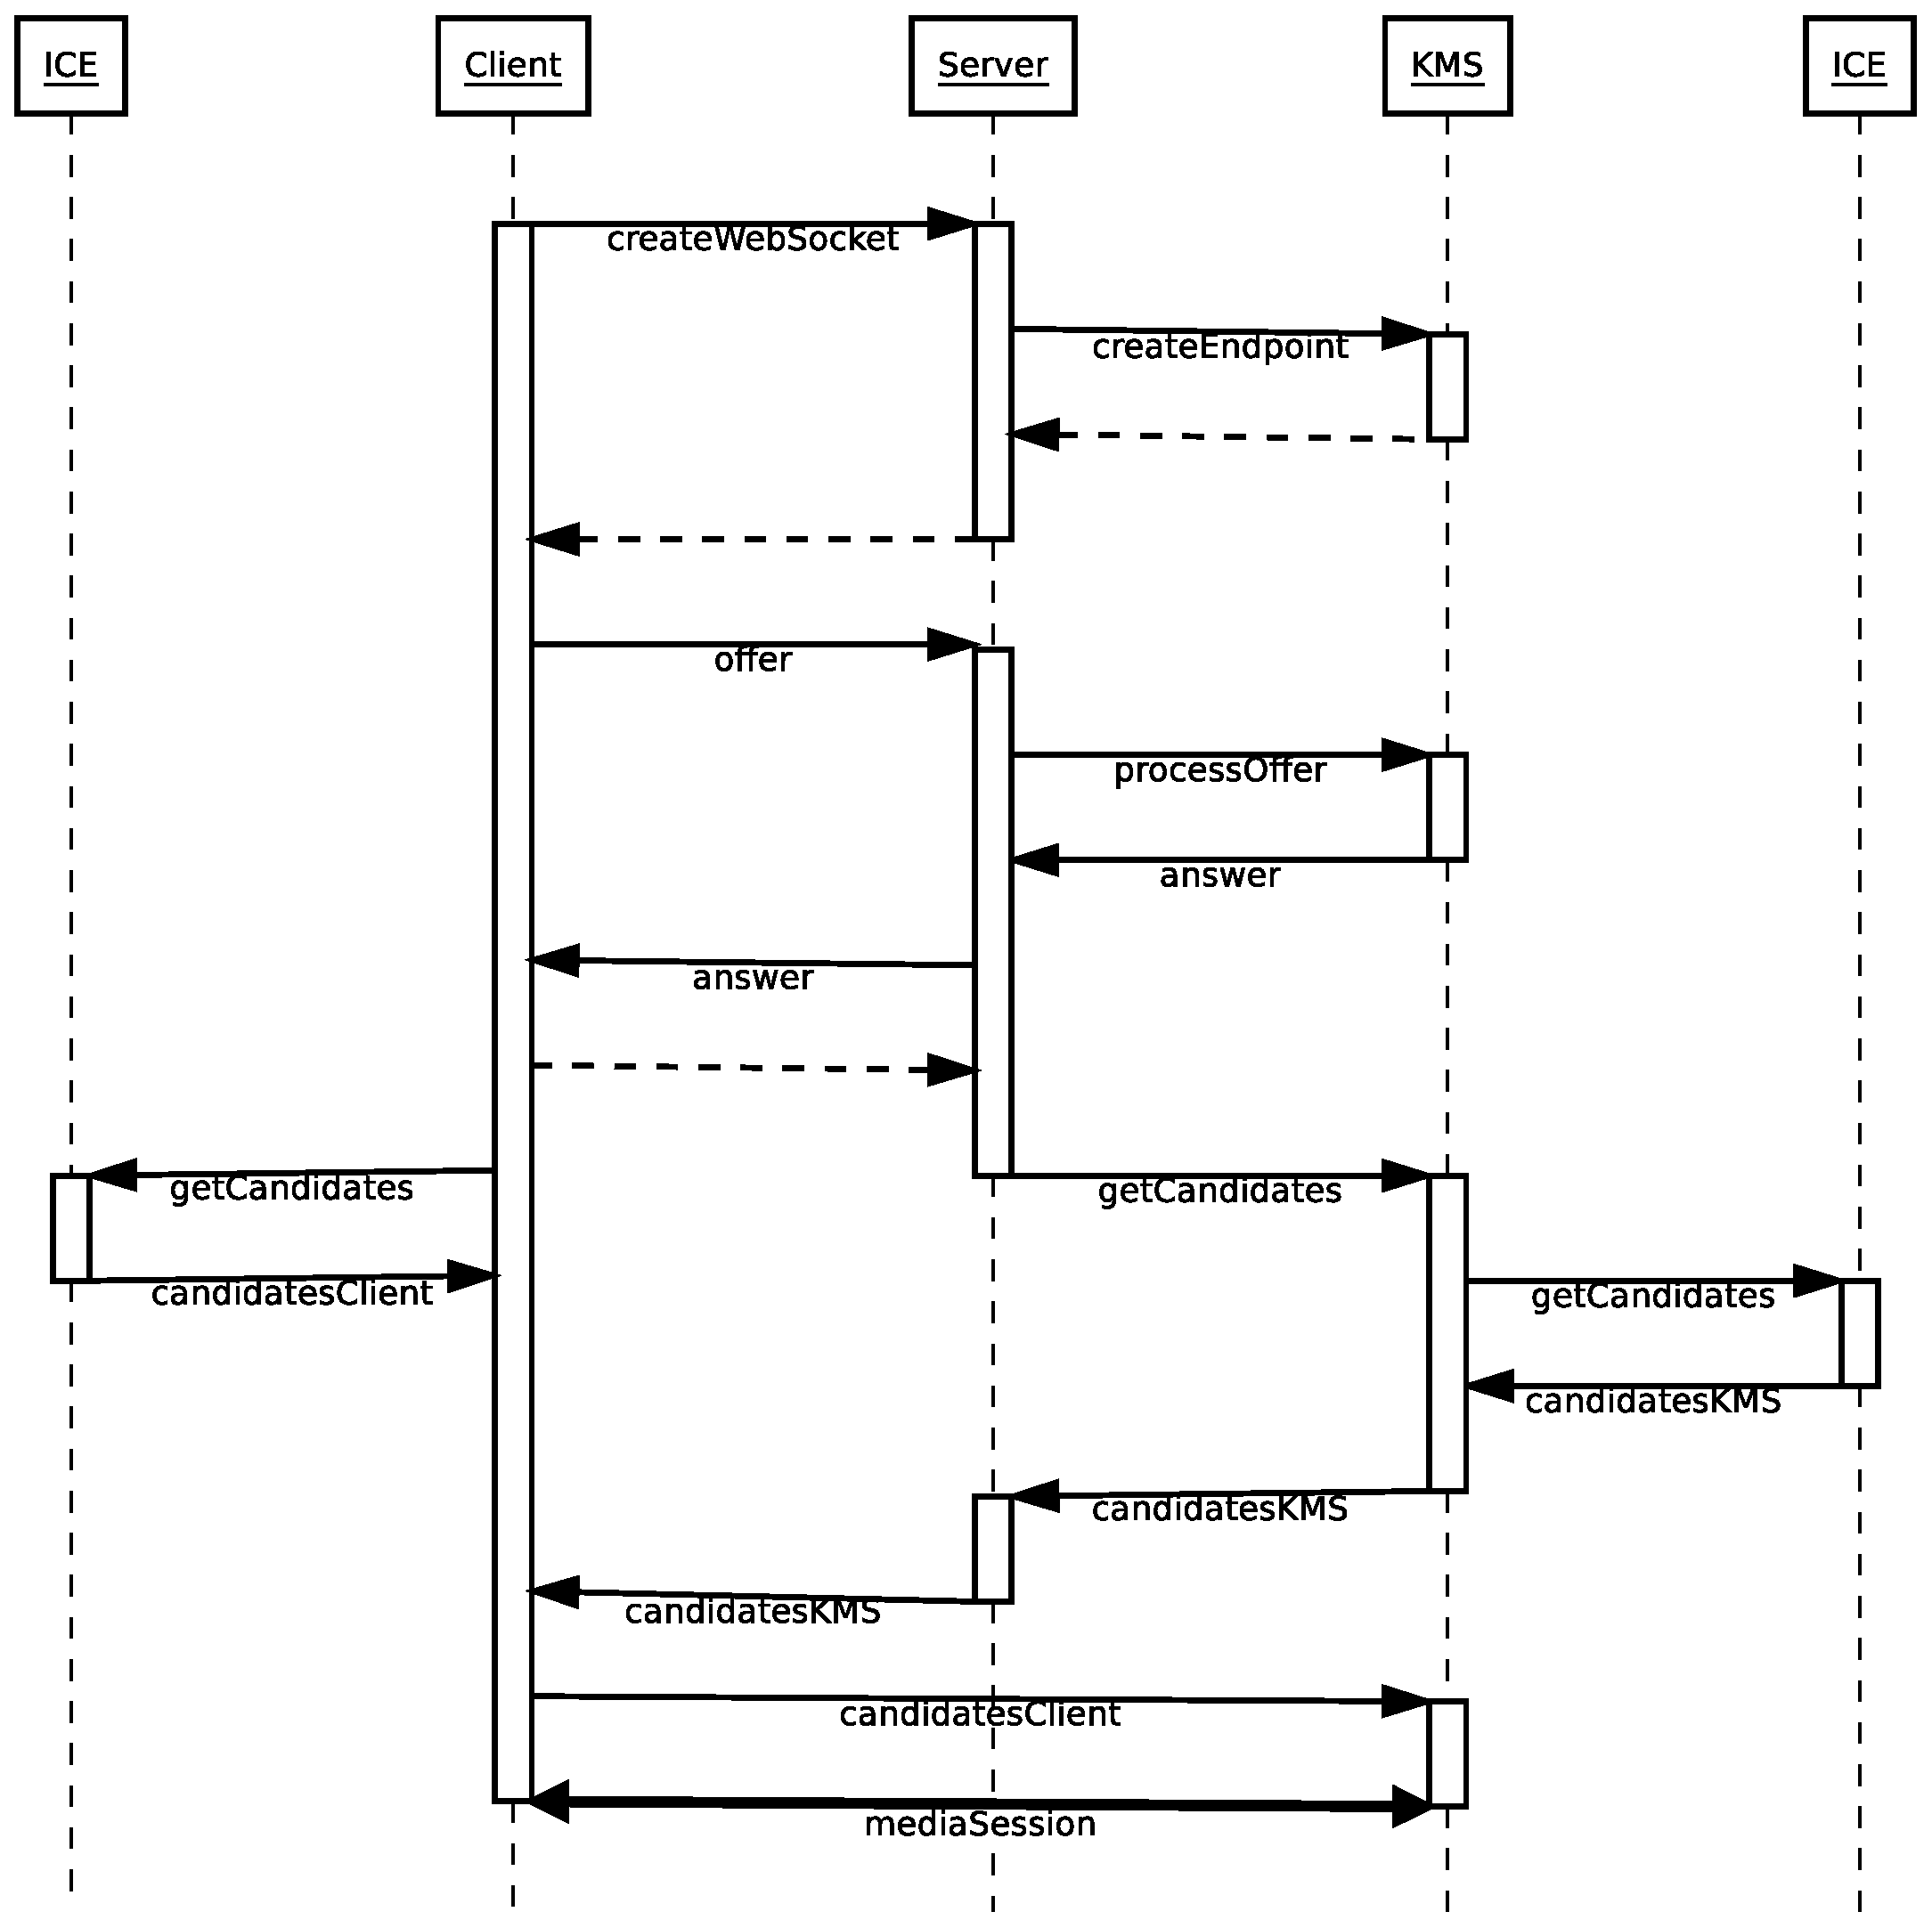
\includegraphics[width=0.9\textwidth]{figures/signaling}
    \end{subfigure}
    \caption{Signaling sequence diagram}
    \label{fig:signaling2}
\end{figure} 


Before the signaling protocol starts, the user must be authenticated. After the user provide the correct credentials, it receives an \ac{HTTP} \emph{cookie} from our server in order to be identified in the following \ac{HTTP} requests.

%RP faz sentido haver dois ICE? Se queres colocar 2 dá-lhes nomes diferentes (nem que seja cliente e servidor ou 1 e 2).

After the web application server validates the user access, the signaling protocol allows the users to directly connect to the \ac{KMS}, which is placed in a private network, and lets the application server and users negotiate media types and encoding information to use during the conversation.
%RP o it em ``it allows'' é quem? webserver ou signaling protocol?
%HR done
We considered implementing the signaling protocol using \ac{HTTP} messages.
However, they would transport extra information such as \ac{HTTP} headers and would follow a request-response signaling mechanism which would not be the best option, as multiple ICE candidates can arrive at any time. Using a \ac{REST} \ac{API} over \ac{HTTP} for signaling and allowing other methods to be called at the same time would lead to opening multiple \ac{TCP} connections at the same time.

Instead, if we create a \emph{WebSocket} \ac{API}, we only need one \ac{TCP} connection and, at the same, provide bi-directional communications without additional headers. Moreover, using \emph{WebSocket} allows the application server to send messages asynchronously to the client without the client having to request it, which can be slightly faster than using \ac{HTTP} which is based on a request followed by a response.
%RP em vez de slighhtly faster não queres antes enfatizar que pode ser antes o servidor a iniciar a comunicação, de forma assincrona?
%HR done
Our signaling protocol consists of sending and receiving \ac{JSON} formated messages, \emph{e.g.} Listing \ref{lst:msgtype}, over WebSockets by both the application server and the client. 

\begin{minipage}{\linewidth}
\begin{lstlisting}[caption={General structure of our WebSocket messages},label={lst:msgtype},language=json]
{
	"cmd":<cmd>,
	"data":<data>
}
\end{lstlisting}
\end{minipage}

When a user enters a group conference, after the page is completely loaded, a WebSocket is created to maintain a connection with our web servers. 
But before creating the web socket, we must identify the user and check if he has permissions to participate in the conference. The user identification is done by retrieving the session id from the cookie provided by the user-agent (web browser) through the \ac{HTTP} headers.
%RP não é bem o user que fornece o cookie. é o user-agent (browser). Convém ser preciso.
%HR done
The web application server retrieves all the information needed from the database in order to check if the user has permissions to join that conference room. It is important to save the user identification before the \emph{WebSocket} connection is created because, after the handshake is performed by the \emph{WebSocket} protocol\cite{rfc6455}, the \ac{HTTP} context is lost.
%RP socket -> websocket?

When the connection is established between the application server and the client, a \emph{PeerConnection} is created on the client and immediately after, an \ac{WebRTC} endpoint is created on the server, specifying a possible set of \ac{ICE} servers to connect.
%RP Usa Application server e não apenas server. Há muitos servers.

At this stage, the web application's user is asked if he wants to share its camera and microphone, share screen or just receive streams from the server. If the user decides to perform a screen share, \emph{adapter.js}\footnote{\url{https://github.com/Temasys/AdapterJS}(accessed March 15, 2016).} may ask to install a plug-in if the browser does not support screen sharing \footnote{\url{http://iswebrtcreadyyet.com/} (Accessed May 11, 2016)}.
%RP web app user? OU apenas client user?
%RP foot note com exemplos de browsers que aceitem screen sharing?
%HR done
If the user decides to share either from camera or screen, \emph{getUserMedia} is called with the correspondent constraints in order to obtain a local stream. We use the constraints presented on Listing \ref{lst:constraints}. 

\begin{minipage}{\linewidth}
\begin{lstlisting}[caption={Media constraints},label={lst:constraints},language=JavaScript]
var screenShareConstraints = {	
	"video": {
		"mediaSource": "window" || "screen"
	}, 
	"audio": false
};
var cameraMicrophoneConstraints = {
	"audio":true, 
	"video":true 
};
var receiveOnlyConstraints = {
	"offerToReceiveAudio":true,
	"offerToReceiveVideo":true
};
\end{lstlisting}
\end{minipage}

If the user decides to share his camera or screen, a pop-up is raised in order to ask the user to give permission to share those resources. If the resources are shared successfully, the user agent creates an offer like Listing \ref{lst:sig01}, sets a \emph{local session description} to its \emph{PeerConnection} and sends it through the WebSocket to the Application Server.
%RP usas ``user'' duas vezes, uma para te referires ao utilizador e outra ao browser (user agent).
If the resources are not shared or the user specified to receive stream only, an \ac{SDP} offer is created specifying the constraints for receiving only video and audio.
%RP offer -> SDP offer?

\begin{minipage}{\linewidth}
\begin{lstlisting}[caption={Offer created by client},label={lst:sig01},language=json]
{
	"cmd":"offer",
	"data":{
		"type":"offer",
		"sdp":<sdp>	// omitted for brevity
	}
}
\end{lstlisting}
\end{minipage}

The \emph{local session description} contains the session identifier, codecs, containers, transport protocols and ports used per media type. The \emph{local session description} is useful to conclude if the client is receiving only, which means that \ac{KMS} does not need to mix, record nor analyze streams coming from the user's \ac{WebRTC} endpoint. 

The server receives and processes the offer and sets the \emph{remote session description} to its client associated \ac{WebRTC} endpoint. Then a \emph{local session description}, like the one presented in Listing \ref{lst:sig02}, is created on the server and sent back to the client. After that, the server tries to gather \ac{ICE} candidates.
%RP listing -> Listing

\begin{minipage}{\linewidth}
\begin{lstlisting}[caption={Answer created by KMS},label={lst:sig02},language=json]
{
	"cmd":"answer",
	"data":{
		"type":"answer",
		"sdp":<sdp>	// omitted for brevity
	}
}
\end{lstlisting}
\end{minipage}

The client receives the server answer, sets the \emph{remote session description} and gets the ice candidates from the \ac{ICE} server.
%RP tens ``ice'', ``\ac{ICE}''. Acho que também já vi ``ICE''. Convém ser sempre igual!

Subsequently, after a while both the server and client receive the \ac{ICE} candidates that allow the client to connect directly to \ac{KMS} and vice-versa. The candidates are received at the client which sets them to its \emph{PeerConnection}. The same is done on the server which receives the \ac{ICE} candidates like on Listing \ref{lst:sig03} from the client and propagates them to \ac{KMS}.
%RP A figura 4.1 precisa de vir antes deste texto todo, para ser mais fácil de perceber.
%RP também tens de explicar porque razão escolheste colocar o KMS numa rede privada. Se está numa rede privada, usas NAT ou um proxy (socket) para estabelecer a ligação?
%HR uso NAT, falei disso na arquitectura, serve para o cliente não aceder directamente ao servidor de streaming e realizar o seu proprio protocolo de sinalizacao (uso indevido por parte de atacantes)

\begin{minipage}{\linewidth}
\begin{lstlisting}[caption={ICE candidates sent by KMS and client},label={lst:sig03},language=json]
{
	"cmd":"iceCandidate",
	"data":{
		"sdpMLineIndex":0,
		"candidate":"candidate:15 1 TCP 843056127 146.193.224.20 48828 typ srflx raddr 192.168.1.105 rport 48828 tcptype passive",
		"sdpMid":"audio"
	},
}
\end{lstlisting}
\end{minipage}

An \ac{ICE} candidate contains an \ac{IP}, port, used transport protocol and an attribute named \emph{sdpMLineIndex} that is used for mapping to the \emph{remote session description} media type.
In addition, both intervenients test the connectivity of each \ac{ICE} candidate. When a connection is established, the user and server start to interchange stream data but other \ac{ICE} candidates may arrive with better connections. When that happens, the connection changes seamlessly. 

Having the media session established, the server starts to record any received stream and the client creates an \ac{URL} correspondent to the stream location.


%RP não falas nada sobre chats, etc! Não há signalling para isso?
%HR não, só video e audio, chat é websockets
\section{Stream Recording}
	In this section we describe our approaches for the stream recording implementation, namely recording on the client side and server side.

\subsection{Client side recording}
	In order to record used shared streams, our first approach consisted on recording video and audio streams into blobs of limited duration. Because each user was recording directly from their shared local resources, we achieved the best stream quality.

	After recording, each block was uploaded to our server through \ac{HTTP} and saved into the file system, the block meta-data was created and inserted on our database. Each block meta-data contained the file's location for the recorded block, the starting date, duration, user identification and group identification. When the file was completely saved the meta-data was advertised to the remaining users. This meta-data was simply used to refresh the user interface, the meta-data was completely discard after that because an huge amount of small blocks meta-data would use more and more memory as time went by. 

	The process to play a video was quite simple, the user specified which user and date was intended to play, the server calculated the intersection between the requested date and the block bounds and returned the file to the client.

	Although this idea was fairly simple, we couldn't achieve seamless sequential block switching. Downloading the video file always toke a noticeable amount of time. To solve this problem while we were playing a block, the next one was downloading in parallel so when the current block finished playing we would have an available block to play. 

	Block switching became more acceptable, but switching the \ac{URL} always produced a flash. We solved this problem by having two layers and set the \ac{URL} to the back layer, the front layer frozen with the last frame, then we changed the back layer to front. 

	After we implemented our recording solution using this approach, we tested locally and remotely. For remote connections we observed a fairly high bandwidth usage mainly because blocks were both sent and received at maximum quality. 

\subsection{Server side recording to file system}

	Before recording any type of stream we had to analyze the user media offer in order to check if a video as really being received by \ac{KMS}, otherwise if we would not verify the user's offer, the recording video would be black.

	The streaming content received on \ac{KMS} was already compressed due to \ac{WebRTC}'s exchanged quality of service metrics data. As a direct consequence our recorder solution used on most cases less disk space per block, but would never use more storage than client side recording. \ac{KMS} allows recording files using \emph{webm} and \emph{mp4} containers.

	With server side recording, the user would maintain always the same stream \ac{URL} even if it is playing real-time video or reproducing recorded video. When a user desires to play recorded video, a \emph{webSocket} message is sent specifying the time and the intended user id, the group identification is not sent because it is already associated to the \emph{webSocket}. The server performs the same calculations in order to find a block that intersects the requested time, plays it and when finished the next part is automatically played without the user intervention.

	We observed differences in image quality when switching parts, that was even noticeable if we set a short block duration. We also noticed a small gap on audio when switching blocks but it was acceptable and speech recognition was not very affected. 

	Back when we were implementing our solution, \ac{KMS} had not support for seeking videos, which meant that blocks would would always start playing from their beginning. This lead to a theoretic playing time error that can be at most half the duration of a block. In practice the maximum playing time error coincides with the block duration because we perform the intersection between the requested date and the block but we could decrease the error by half if we calculate the intersection with the requested time plus half the duration. 

	\begin{figure}
			\centering

	\begin{tikzpicture}[y=1cm, x=1cm, thick, font=\footnotesize]    

		\tikzset{
		   brace_top/.style={
		     decoration={brace},
		     decorate
		   },
		   brace_bottom/.style={
		     decoration={brace, mirror},
		     decorate
		   }
		}

		% time line hour
		\draw[line width=1.2pt, ->, >=latex'](0,-3.0) -- coordinate (x axis) (9,-3.0) node[right] {time}; 
		\foreach \x in {1,2,3,4,5} \draw (\x*1.5,-2.9) -- (\x*1.5,-3.1) node[below] {};

		% top brace
		\draw [brace_top] (1*1.5+0.03,-2.7) -- node [above, pos=0.5] {$ block_{n}$} 	(3*1.5-0.03,-2.7);
		\draw [brace_top] (3*1.5+0.03,-2.7) -- node [above, pos=0.5] {$ block_{n+1}$} 	(5*1.5-0.03,-2.7);

	    \draw  node[fill,circle,scale=0.6]at (2*1.5,-3.0)  {};%

		% low brace period
	
		\draw [brace_bottom] (1*1.5+0.03,-3.3) -- node [below, pos=0.5] {$e_{n}=\frac{d}{2}$} 		(2*1.5-0.03,-3.3);
		\draw [brace_bottom] (2*1.5+0.03,-3.3) -- node [below, pos=0.5] {$e_{n+1}=\frac{d}{2}$} 	(3*1.5-0.03,-3.3);
		\draw [brace_bottom] (3*1.5+0.03,-3.3) -- node [below, pos=0.5] {$d$} 						(5*1.5-0.03,-3.3);

	\end{tikzpicture}
		\caption{Theoretic maximum playing error $(e)$}
	\end{figure}

	\begin{figure}
			\centering
	\begin{tikzpicture}[y=1cm, x=1cm, thick, font=\footnotesize]    

		\tikzset{
		   brace_top/.style={
		     decoration={brace},
		     decorate
		   },
		   brace_bottom/.style={
		     decoration={brace, mirror},
		     decorate
		   }
		}

		% time line hour
		\draw[line width=1.2pt, ->, >=latex'](0,-3.0) -- coordinate (x axis) (9,-3.0) node[right] {time}; 
		\foreach \x in {1,2,3,4,5} \draw (\x*1.5,-2.9) -- (\x*1.5,-3.1) node[below] {};

		% top brace
		\draw [brace_top] (1*1.5+0.03,-2.7) -- node [above, pos=0.5] {$ block_{n}$} 	(3*1.5-0.03,-2.7);
		\draw [brace_top] (3*1.5+0.03,-2.7) -- node [above, pos=0.5] {$ block_{n+1}$} 	(5*1.5-0.03,-2.7);

	    \draw  node[fill,circle,scale=0.6]at (3*1.5,-3.0)  {};%

		% low brace period
	
		\draw [brace_bottom] (1*1.5+0.03,-3.3) -- node [below, pos=0.5] {$e_{n}=d$} 	(3*1.5-0.03,-3.3);
		\draw [brace_bottom] (3*1.5+0.03,-3.3) -- node [below, pos=0.5] {$d$} 		(5*1.5-0.03,-3.3);

	\end{tikzpicture}
		\caption{Practical maximum playing error $(e)$}
	\end{figure}



	For playing video with an higher velocity we used \emph{ffmpeg}\footnote{\url{https://www.ffmpeg.org/}(accessed: 17 March 2016)} to convert the block into a new video with the desired velocity and seek time. Because the media duration is known, when the video started to being convert the headers located at the beginning of the file were already written and that made it possible to stream while converting.

	%{\color{red} [TALK ABOUT COMPLEXITY OF DECODE VS DECODE+MANIPULATE+ENCODE]}

	Although we implemented a solution that worked, we immediately noticed that \emph{ffmpeg} would take some time to initialize and that lead to pauses between switching parts.

	Later the \emph{Kurento} team released a version with support for seeking videos but we had to suspend the implementation of the fast forwarding feature as currently \ac{KMS} is not supporting that.

	We could implement fast forwarding without real time conversion by creating multiple versions of the same video with different velocities after the recording of a block. When a user needed to play he would also need to specify one of the available velocities. We did not followed this approach has it would require a bigger disk space usage. 

\subsection{Server side recording to database}

	One of our concerns during the development of our solution was the storage scalability. Saving files directly into file system would require an extra effort to distribute and replicate files among servers. For that purpose \emph{Kurento} team developed \emph{Kurento Repository}\footnote{\url{http://doc-kurento-repository.readthedocs.org} (accessed on 17 March 2016)} which is based on \emph{MongoDB}.

	One of the features that \emph{Kurento Repository} provides is the ability to play directly from the database without having to download the entire file to \ac{KMS}. The same is true for recording, but because the file headers are in the beginning and the file is written until is stops, the headers don't contain the necessary information for seeking the file.

	Although we gain with scalability with this approach, we lose access over the file for changing it to fit our needs, namely for using \emph{ffmpeg} or other video manipulation tool.

	Although we did not implemented recorded file seeking, that could be achieved by waiting for full file recording and then proceed to database insertion with the correct headers. Another approach would be the specification of the file duration before recording so the correct file headers could be written a priori. Both approaches were not possible to implement using just the \emph{Kurento} clients, we would need change the source code of \emph{Kurento} in order to add those new features.






\section{Hyper Content}
	In this section we describe the algorithm we created to show synchronized interactive content to clients.



	\subsection{Content creation}

	In order to create content the user has the option to write simple movie captions without writing any code, otherwise, as mentioned before, it can write \ac{HTML}, \ac{CSS} and \emph{JavaScript}. The definition of the content's starting and ending time by the user it's not an easy task. Defining the content's time to appear in real-time would require a previous user plan. Otherwise the user could make a speech and add the content for later reproduction.

	Figure \ref{fig:creation} shows the user interface for creating interactive hyper content manually.

	\begin{figure}[H]
		\centering
		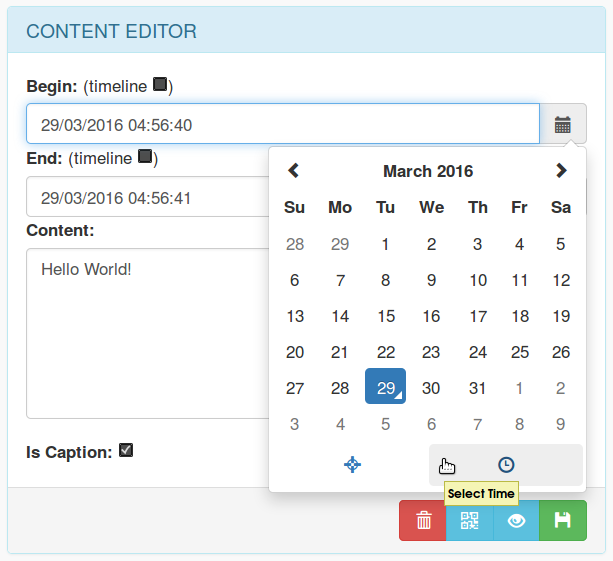
\includegraphics[width=0.6\textwidth]{figures/edition.png}
		\caption{Manual content creation}
		\label{fig:creation}
	\end{figure}


	Listing \ref{lst:createcontent} shows the structure of the content created by one user.

\begin{minipage}{\linewidth}
\begin{lstlisting}[caption={Exampe of content created by one user},label={lst:createcontent},language=json]
{
	"cmd":"createContent",
	"start":"2016-03-29T03:56:40.000Z",
	"end":"2016-03-29T03:56:41.000Z",
	"content":"<h1>Hello</h1>"
}
\end{lstlisting}
\end{minipage}
	In order to help the content creator to show and synchronize its content in real-time we allow the user to encode its content into \emph{QR codes} and show it to the camera in real time.

	\ac{KMS} lets registering event handlers for \emph{QR code} detection. The component that detects \emph{QR codes} on \ac{KMS} is called periodically and fires the handlers with the decoded content. This mechanism does not detect if the \emph{QR code} enters or leaves the screen. We had to implement our own mechanism for detecting those events.

	Each user session in the server maintains a map with the contents that are present on the screen. In order to apply our algorithm more efficiently we calculate the content's hash through the \emph{md5} method.

	If the hash is not present in the map it means the \emph{QR code} was entering the screen, we add that hash to the map and associate the current time to it, all the users are notified to watch that content in real-time. By doing an analogy to the \emph{Nyquist} theorem we know that if the same \emph{QR code} is not detected after a time bigger then two periods we can conclude that the \emph{QR code} leaved the screen and we add the correspondent content into our database. Listing \ref{lst:pseudo_qrcode} shows the pseudo code for \emph{QR code} leaving detection.

\begin{minipage}[!htb]{\linewidth}
\begin{lstlisting}[caption={Pseudo code for QR code leaving detection},label={lst:pseudo_qrcode},language=JavaScript]
var ongoingCodesMap = {};
function onCodeFound(content) {
	var startingTime = getCurrentTime() - getUserOffset();
	var hash = md5(content);
	if(ongoingCodesMap[hash] == null){
		sendQRCodeToEditingUser(hash,content);
	}
	ongoingCodesMap[hash] = startingTime;
	waitTwoSeconds(); // onCodeFound() may be called from other threads
	var newestTime = ongoingCodesMap[hash]; 
	if(newestTime == startingTime){
		var endingTime = getCurrentTime() - getUserOffset();
		ongoingCodesMap[hash] = null; 
		sendQRCodeToEditingUser(hash,null); // remove from UI
		insertContentIntoDatabase(startingTime,endingTime,content);
		sendContentToUsers(startingTime,endingTime,content);
	}
}
\end{lstlisting}
\end{minipage}


	Our main content synchronization mechanism is time based but with some programming knowledge it is possible to insert \emph{JavaScript} code that fires events on user interaction. For example, after a teacher's lecture, it is possible to show a quiz to the users in order to understand what they learned and then submit the data to the server for further analysis.


	\subsection{Synchronization}

	In our solution content is represented as simple text that can contain \ac{HTML}, \ac{CSS} or even \emph{JavaScript}, this content is displayed on defined intervals of time.

	Multiple contents can be displayed at the same time, in order to achieve that, we define layers above the video with the same size. Each layer is associated to the content.

	We have taken into account that the amount of content tends to grow with time and the user should only have access to a subset of content instead all of them, which would be very inefficient.

	The content to display for each user depends on the user's position on the time-line, this position is given by an offset between the current time and the navigated time. If the user is watching the content in real-time this offset is constant so there is no need to synchronize this value.

	Each content is divided into two components, the \emph{start} and the \emph{end} which are sent to users. The \emph{start} component contains a time stamp, the content identification number and the content itself in form of text. The \emph{end} component only contains the time stamp and the content identification number. 

	The content to return is given by the union of two content subsets:
	\begin{itemize}
		\item The intersection of the content interval and user's time.
		\item A subset of contents which starting time is immediately following the user's time.
	\end{itemize}

	The second subset is used for predicting which content the user will watch and avoid requests during its events.

	The content description messages that are sent to each user contains the constant itself on the form of a list of events and an attribute that specifies if the server has more content to return.

	Listing \ref{lst:sentcontent} shows the structure of the content sent to users.

\begin{minipage}{\linewidth}
\begin{lstlisting}[caption={Exampe of content sent to users},label={lst:sentcontent},language=json]
{
	"cmd":"content",
	"data":[{
			"id":"56f9fd1aa986c615fab43d69",
			"time":"2016-03-29T03:56:40.000Z",
			"type":"start",
			"content":"<h1>Hello</h1>"
		},{
			"id":"56f9fd1aa986c615fab43d69",
			"time":"2016-03-29T03:56:41.000Z",
			"type":"end"
		}
	],
	"more":false
}
\end{lstlisting}
\end{minipage}

	When a user enters the conference room, immediately after the \emph{WebSocket} creation the server sends him the current content.

	The user receives the content, sorts all components by time and creates a set of events. All the events before the user's time are rendered and removed from the set of events. A timer is scheduled for the first component on the event set and the process repeats while the set is not empty.

	If the set is empty, there two options, if the server contained more content a new request for content is made and the process starts from the beginning, namely the server sends the correspondent content again. If the server has no more content the process is stopped until it sends more.

	The users will receive their contents from the server on five different situations:

	\begin{itemize}
		\item Conference room entrance (advertised by server).
		\item Set of events empty and server has more content (client requested).
		\item Content is created (advertised by server).
		\item Content is removed (advertised by server).
		\item User navigates to different point in time (client requested).
	\end{itemize}



	Listing \ref{lst:pseudo_render} presents the pseudo code for our content scheduler.

\begin{minipage}[!htb]{\linewidth}
\begin{lstlisting}[caption={Pseudo code for hyper content scheduler},label={lst:pseudo_render},language=JavaScript]
function scheduleContent() {
    var navigatedTime = getCurrentTime() - getUserOffset();
    while ( hasLocalEvents() ) {
        if ( firstEventIsOlderThanNavigatedTime() ) {
            if ( firstEventIsStart() ) {
            	addHtmlLayer(event);
            } else {
            	removeHtmlLayer(event);
            }
            removeFirstEvent();
        } else {
            break;
        }
    }
    if ( hasNoLocalEvents() ) {
    	return;	// nothing to do
    } 
    if ( hasNoStartEvents() && serverHasMoreContent() ) { 
       	requestContentFromServer(navigatedTime);
    } else {
        waitUntilNextEvent();
        scheduleContent();
    }
}
\end{lstlisting}
\end{minipage}

	\subsection{Security Concerns}

	Our solution is flexible on what kind of interactions are possible to the users in real time but allowing users to write \emph{JavaScript} that is executed on the other users browser would attackers to misuse their resources and access to critical information.

	We could solve this problem easily by escaping any \emph{script} tag present on the content, but we would sacrifice the kind of interactions that are possible. 

	By not allowing \emph{JavaScript} we would need to implement all actions a priori and fire them when a type of message is received. We decided to ignore the security vulnerabilities that are exposed by evaluating \emph{JavaScript} because in order to offer the same interactions we would have to do an exhaustive functional requirements gathering.

	Another way to solve this problem, which is not within the goals of this thesis, is to analyze the \emph{JavaScript} code and detect if it is malicious.

	\subsection{Time Manipulation}

	We have used \emph{vis.js} to display out time-line. This library was created for content navigation through time, but it was not designed to be always moving automatically, we have created a background timer that performs the animation of moving the window of time bounds and user navigated time marker.

	Figure \ref{fig:timeline} shows the the graphic appearance of our interactive time-line, in order to navigate through time the user must drag and drop the time-line horizontally, when the user drops the time-line an event handler is called with the new user's time offset which will be used to send a message to the server in order to choose the correspondent content to display. 

	\begin{figure}[!htb]
		\centering
		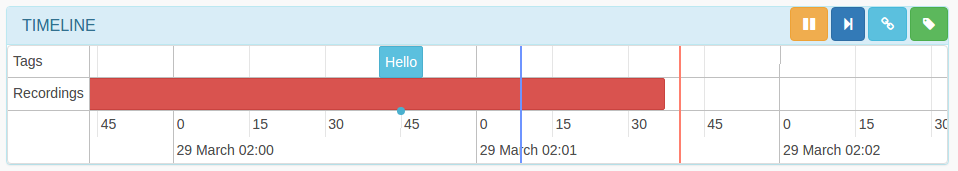
\includegraphics[width=\textwidth]{figures/timeline.png}
		\caption{Interactive time-line}
		\label{fig:timeline}
	\end{figure}

	We have noticed the server time being different from client time and this created graphic inconsistencies such as showing existing recorded blocks of movie in the future. To solve this problem the server sends its time to client immediately after the \emph{webSocket} creation, we synchronize the time-line with the server and although it may exist a small error due to network transmission time the graphical error is negligible. 


	\subsection{Time annotations creation}

	Time annotations are simpler way save points in time and share them with other users. When a user enters in a conference room the server sends all annotations so they can be displayed directly into the user time-line. Each time annotation is created all users are advertised so they can update their interfaces.

	Figure \ref{fig:annotation} shows the creation and placement of annotations on the time-line, to save the annotation the user must click on the floppy icon in order to save it and advertise the conference participants. 

	\begin{figure}[!htb]
		\centering
		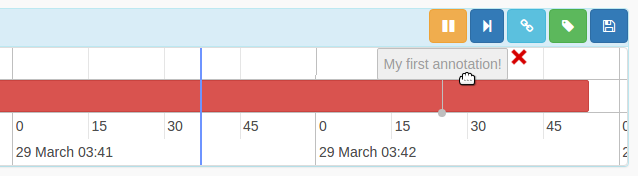
\includegraphics[width=0.7\textwidth]{figures/annotation.png}
		\caption{Creating a time annotation}
		\label{fig:annotation}
	\end{figure}

	Besides the ability to create tags it is also possible to create time hyper-links, see figure \ref{fig:timelink}, that can be sent to other users externally so they can navigate directly to the content when entering in the conference room.


	\begin{figure}[!htb]
		\centering
		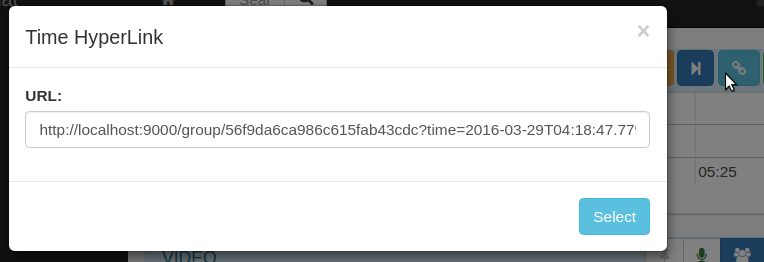
\includegraphics[width=0.8\textwidth]{figures/timelink.png}
		\caption{Time link creation}
		\label{fig:timelink}
	\end{figure}


	\subsection{Content Search}

	Users can easily search for annotations and contents and travel to their correspondent times. In the case of hyper content after handling the result from database we ignore \ac{HTML} tags, extract the text with \emph{Jsoup}\footnote{\url{http://jsoup.org/} (Accessed 21 March 2016)} and apply the query again. We extract the text from \ac{HTML} because accidentally searching for text contained in \ac{HTML} tags would lead to incorrect results.

	Figure \ref{fig:search} shows how the search results are displayed to the user. Each result entry contains an icon specifying the type of result (hyper content, time annotation, ...).




\begin{figure}[!htb]
\centering
\begin{minipage}[b]{0.55\linewidth}
\centering

		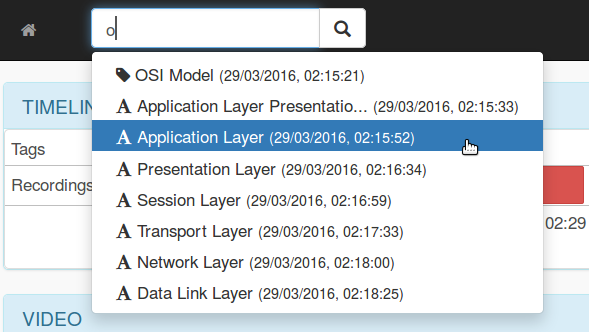
\includegraphics[width=\textwidth]{figures/search.png}
	      a) Result list
\label{fig:minipage1}
\end{minipage}
\quad
\begin{minipage}[b]{0.40\linewidth}
		\centering

		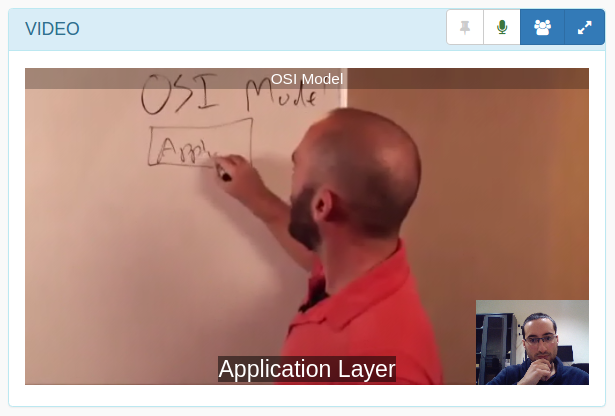
\includegraphics[width=\textwidth]{figures/search2.png}
	       b) Selected result
\label{fig:minipage2}
\end{minipage}

		\caption{Example of search results}
		\label{fig:search}
\end{figure}

	\subsection{Switching views}

		We provide a way for users to select the composite view of the conference room or the video shared by a particular user device as it can be seen on figure \ref{fig:devices}. 

		In order to maintain a list of available user devices that can be played at the navigated time if a user plays or ends playing a block of recorded video it obtains at the same time a list of all devices available for each user at that time.

		On the other hand, if a user changes to real time, the list of devices is extracted from the set of \emph{webSockets} that are associated to the respective conference room. This list of devices is also sent to the users that are also in real time mode whenever a new user enters or leaves the conference room.

	\begin{figure}[!htb]
		\centering
		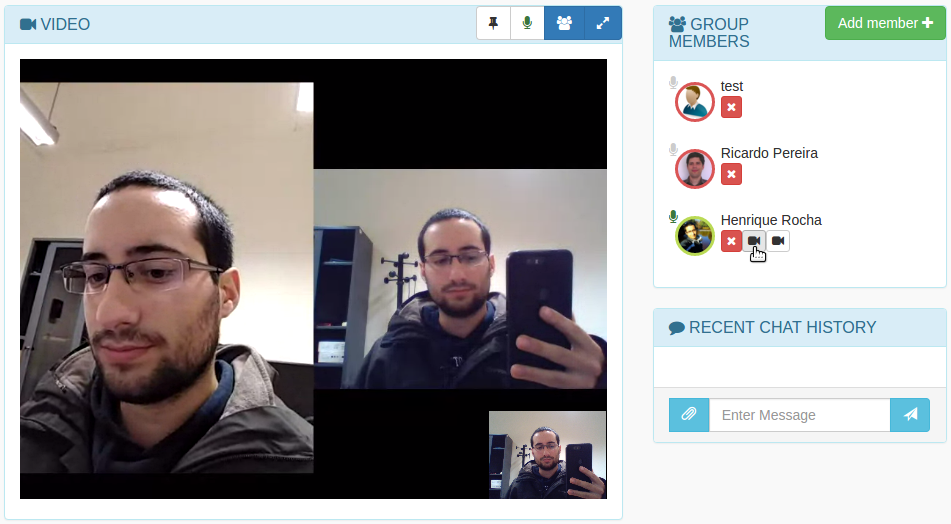
\includegraphics[width=0.8\textwidth]{figures/devices.png}
		\caption{Multiple devices per user}
		\label{fig:devices}
	\end{figure}

		We also provide an automatic mechanism for switching the view to the current speaker. With respect to sound analysis, the sound samples are analyzed on the client side through the web audio \ac{API}.

		Our speech detector is straightforward, we could perform a spectral analysis in order to understand if the analyzed sound contains frequencies in the range of the human voice but instead we just capture sound samples in real time and calculate the maximum sound amplitude. If a sound sample has an amplitude bigger than a factor of the maximum amplitude (we have used an empirical value of 10\%) we say that the user is speaking and therefore we send a message to the server if the speaking state has changed. Subsequently, the server receives the user speaking state and sends it to the other users so they can request a different view.
\section{Chapter Summary}
\label{implementation:summary}

In this chapter we have described how we implemented the various components present on our architecture, the challenges that we have faced and the solutions we have found.

We started by defining the database model, which influenced directly our system's behavior and the extensibility to new functionalities.

Then, we underlined the requirements of our signaling protocol and, as a consequence, we have described, in detail, the protocol itself.

With the signaling protocol implemented, we observed the first outcomes of using \ac{WebRTC}, the basic functionality we have implemented was an echo of the video and audio sent by users. However we have implemented other features such as switching to other user streams, recording and mixing multiple streams into a single one.

In respect to hyper-content, we have described how to create and search for content either being superimposed content to video and time annotations. In relation to displaying content to users we have also defined how we have synchronized the content to show and the security concerns of our choices.

Then, we have described how we have implemented our chat and collaborative editor.


